\subsection{Version}

En esta sección estudiamos el analizador generado por Jison:
\begin{verbatim}
[~/Dropbox/src/javascript/PLgrado/jison-aSb(develop)]$ jison --version
0.4.2
\end{verbatim}

\subsection{Gramática Inicial}
Veamos el módulo generado por jison para esta gramática:
\begin{verbatim}
[~/srcPLgrado/aSb(develop)]$ cat aSb.jison 
%lex
%%
.               { return yytext; }
/lex
%%
S: /* empty */  { console.log("empty"); }
   | 'a' S 'b'  { console.log("S -> aSb"); }
;
%%
\end{verbatim}

% edit chapter_bottomup/aSb.tex
\subsection{Tablas}
Esta es la primera parte del parser generado:
\begin{verbatim}
/* parser generated by jison 0.4.2 */
var aSb = (function() {
    var parser = {
        trace: function trace() {},
        yy: {},
        symbols_: {
            "$accept": 0, /* super-arranque $accept -> S */
            "$end": 1     /* end of input */
            "error": 2, /* numero para el símbolo 'error' */
            "S": 3,     /* numero para el símbolo 'S' */
            "a": 4,
            "b": 5,
        },
        /* array inverso de terminales */
        terminals_: {   /* numero -> terminal */
            2: "error", 
            4: "a",
            5: "b"
        },
        productions_: 
        [0, 
/* 1 */     [3, 0], /* S : vacio        simbolo,longitud de la parte derecha */
/* 2 */     [3, 3]  /* S : a S b        simbolo,longitud */
        ],
\end{verbatim}

\begin{center}
\begin{latexonly}
\begin{figure}[htb]
%\centerline{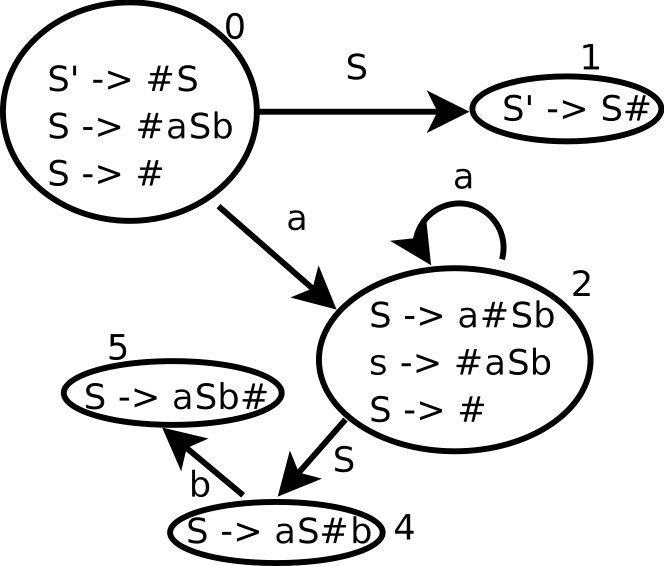
\includegraphics[scale=1.2]{chapter_bottomup/dfa.png}}
\centerline{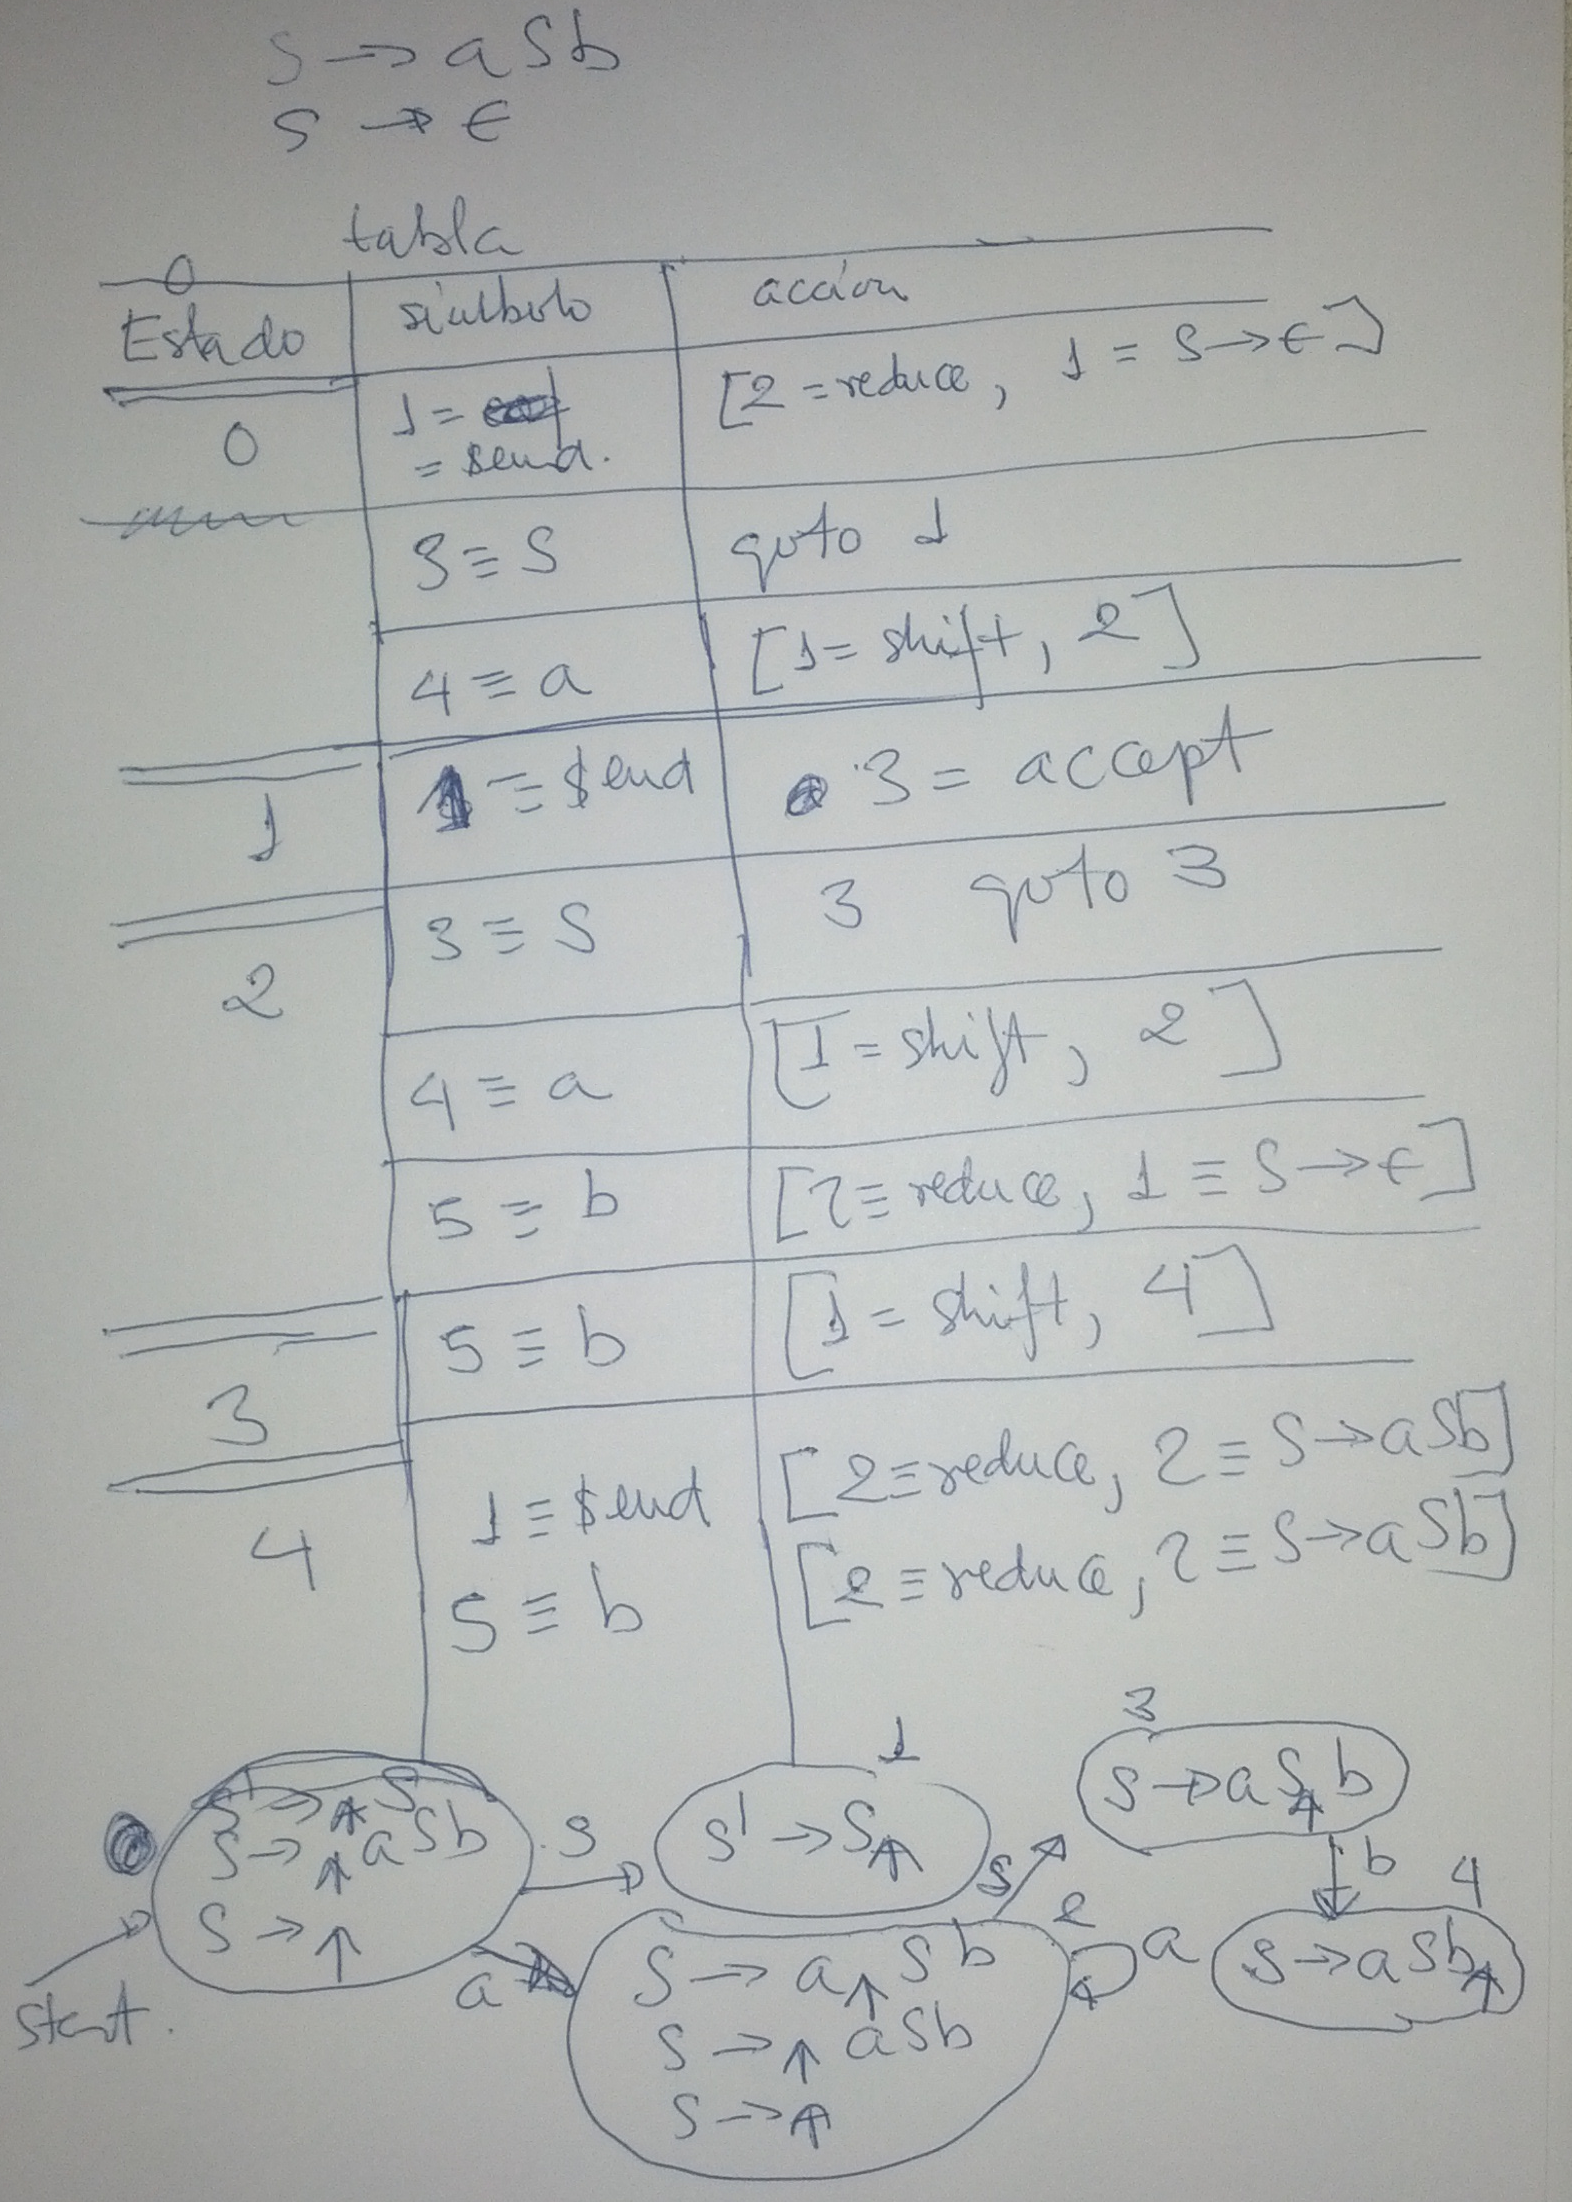
\epsfig{file=chapter_bottomup/aSb.eps, width=12cm}}
\caption{DFA construido por Jison}
\label{fig:dfa}
\end{figure}
\end{latexonly}
\begin{rawhtml}
<img src="aSb.png" width="50%"/>
<p>

DFA construido por Jison
\end{rawhtml}
\end{center}

\subsection{Acciones Semánticas}
Cada vez que se produce una acción de reducción esta función es llamada:
\begin{verbatim}
performAction: function anonymous(yytext, yyleng, yylineno, yy, yystate, $$, _$) {

    var $0 = $$.length - 1;
    switch (yystate) { /* yystate: numero de regla de producción */
        case 1:
            console.log("empty");
            break;
        case 2:
            console.log("S -> aSb");
            break;
    }
},
\end{verbatim}
\begin{itemize}
\item
Parece que  cuando se llama a este método \verb|this| refiere a un objeto \verb|yyval|. Este es el
punto  de llamada a la acción semántica dentro del parser generado por Jison.
Puede encontrarse dentro del parser en el caso de un \verb|switch| 
que corresponde a la acción de reducción:
\begin{verbatim}
r = this.performAction.call(yyval, yytext, yyleng, yylineno, this.yy, action[1], vstack, lstack);
\end{verbatim}
El método \verb|call|
nos permite invocar una función como si fuera un método de algún otro 
objeto. Véase la sección 
\ref{subsection:callyapply}.

Este objeto \verb|yyval| tiene dos atributos: \verb|$| y \verb|_$|.
  \begin{itemize}
  \item
  El atributo 
  \verb|$| se corresponde con \verb|$$| de la gramática (atributo de la variable
  sintactica en la parte izquierda)
  \item
  El atributo \verb|_$| guarda información
  sobre la posición del último token leído.
  \end{itemize}
\item
\verb|yytext| parece contener el texto asociado con el token actual
\item
\verb|yyleng| es la longitud del token actual
\item
\verb|yylineno| es la línea actual (empezando en 0)
\item
\verb|yy| es un objeto con dos atributos \verb|lexer| y \verb|parser| 
\item
\verb|yystate| es el estado actual 
\item
\verb|$$| parece ser un array/pila conteniendo 
los valores de los atributos asociados con los estados de la pila (\verb|vstack| ¿Por value stack?)
\item
Asi pues \verb|$0| es el índice en \verb|$0| del último elemento de \verb|$$|.
Por ejemplo, una acción semántica asociada con una regla \verb|A : B C D| con tres elementos como:
\begin{verbatim}
$$ = $1 + $2 + $3;
\end{verbatim}
Se traduce por:
\begin{verbatim}
this.$ = $$[$0 - 2] + $$[$0 - 1] + $$[$0];
\end{verbatim}
\item
\verb|_$|
Es un array con la información sobre la localización de los simbolos (\verb|lstack| ¿Por location stack?)
\end{itemize}

\subsection{Tabla de Acciones y GOTOs}

\begin{verbatim}
        table: [{
/* 0 */     1: [2, 1],    /* En estado 0 viendo $end(1) reducir por S : vacio */
            3: 1,         /* En el estado 0 viendo S(3) ir al estado 1 */
            4: [1, 2]     /* Estado 0 viendo a(4) shift(1) al estado 2 */
        }, {
/* 1 */     1: [3]        /* En 1 viendo $end(1) aceptar */
        }, {
/* 2 */     3: 3,         /* En 2 viendo S ir a 3 */
            4: [1, 2],    /* En 2 viendo a(4) shift a 2 */
            5: [2, 1]     /* En 2 viendo b(5) reducir por regla 1: S -> vacio */
        }, {
/* 3 */     5: [1, 4]     /* En 3 viendo b(5) shift a 4 */
        }, {
/* 4 */     1: [2, 2],    /* En 4  viendo $end(1) reducir(2) por la 2: S -> aSb */
            5: [2, 2]     /* En 4 viendo b(5) reducir por la 2: S-> aSb */
        }],
\end{verbatim}

\begin{itemize}
\item
La tabla es un array de objetos
\item
El índice de la tabla es el estado. En el ejemplo tenemos 5 estados
\item
El objeto/hash que es el valor contiene las acciones ante los símbolos.
\begin{enumerate}
\item
Los atributos/claves son los símbolos, los valores las acciones
\item
Las acciones son de dos tipos:
\begin{enumerate}
\item
El número del estado al que se transita mediante la tabla \verb|goto|
cuando el símbolo es una variable sintactica 
\item
Un par \verb|[tipo de acción, estado o regla]|. 
Si el \verb|tipo de acción| es 1 indica un shift al \verb|estado| con ese número.
Si el \verb|tipo de acción| es 2 indica una reducción por la \verb|regla| con ese número.
\end{enumerate}
\item
Por ejemplo \verb|table[0]| es 
\begin{verbatim}
        {
            1: [2, 1],    /* En estado 0 viendo $end(1) reducir(2) por S : vacio */
            3: 1,         /* En el estado 0 viendo S(3) ir (goto) al estado 1 */
            4: [1, 2]     /* Estado 0 viendo a(4) shift(1) al estado 2 */
        } 
\end{verbatim}
\end{enumerate}


\end{itemize}

\subsection{defaultActions}
\begin{verbatim}
        defaultActions: {},
\end{verbatim}


\begin{itemize}
\item
\verb|defaultActions| contiene las acciones por defecto.

\item
Después de la construcción de la tabla, Jison identifica para
cada estado la reducción que tiene el conjunto 
de lookaheads mas grande. Para reducir el tamaño del parser,
Jison puede decidir suprimir dicho conjunto y asiganr esa reducción como 
acción del parser por defecto. Tal reducción se conoce como
\cei{reducción por defecto}.
\item Esto puede verse en este segmento del código del parser:
\begin{verbatim}
    while (true) {
          state = stack[stack.length - 1]; 
          if (this.defaultActions[state]) {
              action = this.defaultActions[state];
          } else {
              if (symbol === null || typeof symbol == "undefined") {
                  symbol = lex();
              }   
              action = table[state] && table[state][symbol];
          }   
          ...
    }
\end{verbatim}
\end{itemize}

\subsection{Reducciones}
\begin{verbatim}
parse: function parse(input) {
    ...
    while (true) {
        state = stack[stack.length - 1];
        if (this.defaultActions[state]) {
            action = this.defaultActions[state];
        } else {
            if (symbol === null || typeof symbol == "undefined") {
                symbol = lex(); /* obtener siguiente token */
            }
            action = table[state] && table[state][symbol];
        }
        if (typeof action === "undefined" || !action.length || !action[0]) {
          ... // error
        }
        if (action[0] instanceof Array && action.length > 1) {
            throw new Error("Parse Error: multiple actions possible at state: ..." 
        }
        switch (action[0]) {
            case 1:                                    // shift
                ...
                break;
            case 2:                                    // reduce
                len = this.productions_[action[1]][1]; // longitud de la producción
                yyval.$ = vstack[vstack.length - len];
                yyval._$ = {                           // datos de la posición
                    first_line: lstack[lstack.length - (len || 1)].first_line,
                    last_line: lstack[lstack.length - 1].last_line,
                    first_column: lstack[lstack.length - (len || 1)].first_column,
                    last_column: lstack[lstack.length - 1].last_column
                };
                ...
                r = this.performAction.call(yyval, yytext, yyleng, yylineno, this.yy, action[1], vstack, lstack);
                if (typeof r !== "undefined") {
                    return r; /* un return de algo distinto de undefined nos saca del parser */
                }
                if (len) {                                  /* retirar de las pilas */
                    stack = stack.slice(0, - 1 * len * 2);  /* simbolo, estado, simbolo, estado ... */
                    vstack = vstack.slice(0, - 1 * len);    /* retirar atributos */
                    lstack = lstack.slice(0, - 1 * len);    /* retirar localizaciones */
                }
                stack.push(this.productions_[action[1]][0]); /* empujemos el símbolo */
                vstack.push(yyval.$);                        /* empujemos valor semantico */
                lstack.push(yyval._$);                       /* empujemos localización */
                newState = table[stack[stack.length - 2]][stack[stack.length - 1]];
                stack.push(newState);                        /* empujemos goto[top][A]*/
                break;
            case 3: // accept
                return true;
        }
    }
    return true;
}
\end{verbatim}

\subsection{Desplazamientos/Shifts}

\begin{verbatim}
parse: function parse(input) {
    ...
    while (true) {
        state = stack[stack.length - 1];     /* estado en el top de la pila */
        if (this.defaultActions[state]) {    /* definida la acción por defecto? */
            action = this.defaultActions[state];
        } else {
            if (symbol === null || typeof symbol == "undefined") {
                symbol = lex();              /* obtener token */
            }
            action = table[state] && table[state][symbol]; /* obtener la acción para el estado actual */
        }
        if (typeof action === "undefined" || !action.length || !action[0]) { 
            ... /* error */
        }
        if (action[0] instanceof Array && action.length > 1) {
            throw new Error("Parse Error: multiple actions possible at state: " + state + ", token: " + symbol);
        }
        switch (action[0]) {
            case 1:
                stack.push(symbol);                /* empujamos token */
                vstack.push(this.lexer.yytext);    /* empujamos el atributo del token */
                lstack.push(this.lexer.yylloc);    /* salvamos la localización del token */
                stack.push(action[1]);             /* salvamos el estado */
                symbol = null;
                if (!preErrorSymbol) {             /* si no hay errores ... */
                    yyleng = this.lexer.yyleng;    /* actualizamos los atributos */
                    yytext = this.lexer.yytext;    /* del objeto */
                    yylineno = this.lexer.yylineno;
                    yyloc = this.lexer.yylloc;
                    if (recovering > 0) recovering--; /* las cosas van mejor si hubieron errores */
                } else {
                    symbol = preErrorSymbol;
                    preErrorSymbol = null;
                }
                break;
            case 2:
                ...
                break;
            case 3:
                return true;
        }
    }
    return true;
}
\end{verbatim}

\subsection{Manejo de Errores}

\begin{verbatim}
while (true) {
    state = stack[stack.length - 1];
    if (this.defaultActions[state]) { action = this.defaultActions[state]; } 
    else {
        if (symbol === null || typeof symbol == "undefined") { symbol = lex(); }
        action = table[state] && table[state][symbol];
    }
    if (typeof action === "undefined" || !action.length || !action[0]) {
        var errStr = "";
        if (!recovering) { /* recovering = en estado de recuperación de un error */
            expected = [];                       /* computemos los tokens esperados */
            for (p in table[state])              /* si el estado "state" transita con p */
              if (this.terminals_[p] && p > 2) { /* y "p" es un terminal no especial */
                  expected.push("'" + this.terminals_[p] + "'"); /* entonces es esperado */
              }
            if (this.lexer.showPosition) { /* si esta definida la función showPosition */
                errStr = "Parse error on line " + (yylineno + 1) + 
                         ":\n" + this.lexer.showPosition() + 
                         "\nExpecting " + expected.join(", ") + 
                         ", got '" + 
                         (this.terminals_[symbol] || symbol) + /* terminals_ es el array inverso */
                         "'";                                  /* numero -> terminal             */
            } else { /* ¡monta la cadena como puedas! */
                errStr = "Parse error on line " + (yylineno + 1) + 
                         ": Unexpected " + 
                         (symbol == 1 ? "end of input" : "'" + 
                         (this.terminals_[symbol] || symbol) + "'");
            }
            this.parseError(errStr, {    /* genera la excepción */
                text: this.lexer.match,  /* hash/objeto conteniendo los detalles del */
                token: this.terminals_[symbol] || symbol,                   /* error */
                line: this.lexer.yylineno,
                loc: yyloc,
                expected: expected
            });
        }
    }
    if (action[0] instanceof Array && action.length > 1) {
        throw new Error("Parse Error: multiple actions possible at state: " + state + ", token: " + symbol);
    }
    ...
}
\end{verbatim}

La función \verb|parseError| genera una excepción:

\begin{verbatim}
        parseError: function parseError(str, hash) {
            throw new Error(str); /* El hash contiene info sobre el error: token, linea, etc. */
        },
\end{verbatim}

\begin{itemize}
\item
\verb|parseError| es llamada cada vez que ocurre un error sintáctico.
\verb|str| contiene la cadena con el mensaje de error del tipo: 
\verb|Expecting something, got other thing'|.
\verb|hash| contiene atributos como \verb|expected|: el array de tokens esperados; 
\verb|line| la línea implicada, \verb|loc| una descripción de la localización detallada del punto/terminal
en el que ocurre el error; etc.
\end{itemize}


\subsection{Analizador Léxico}
El analizador léxico:
\begin{verbatim}
/* generated by jison-lex 0.1.0 */
var lexer = (function() {
    var lexer = {
        EOF: 1,
        parseError: function parseError(str, hash) { /* manejo de errores léxicos */ },
        setInput: function(input) { /* inicializar la entrada para el analizadorléxico */},
        input: function() { /* ... */ },
        unput: function(ch) { /* devolver al flujo de entrada */ },
        more: function() { /* ... */ },
        less: function(n) { /* ... */ },
        pastInput: function() { /* ... */ },
        upcomingInput: function() { /* ... */ },
        showPosition: function() { /* ... */ },
        next: function() {
                if (this.done) { return this.EOF; }
                if (!this._input) this.done = true;

                var token, match, tempMatch, index, col, lines;
                if (!this._more) { this.yytext = ''; this.match = ''; }
                var rules = this._currentRules();
                for (var i = 0; i < rules.length; i++) {
                    tempMatch = this._input.match(this.rules[rules[i]]);
                    if (tempMatch && (!match || tempMatch[0].length > match[0].length)) {
                        match = tempMatch;
                        index = i;
                        if (!this.options.flex) break;
                    }
                }
                if (match) {
                    lines = match[0].match(/(?:\r\n?|\n).*/g);
                    if (lines) this.yylineno += lines.length;
                    this.yylloc = {
                        first_line: this.yylloc.last_line,
                        last_line: this.yylineno + 1,
                        first_column: this.yylloc.last_column,
                        last_column: 
                          lines ? lines[lines.length - 1].length - 
                                  lines[lines.length - 1].match(/\r?\n?/)[0].length 
                                  : 
                                  this.yylloc.last_column + match[0].length
                    };
                    this.yytext += match[0];
                    this.match += match[0];
                    this.matches = match;
                    this.yyleng = this.yytext.length;
                    if (this.options.ranges) {
                        this.yylloc.range = [this.offset, this.offset += this.yyleng];
                    }
                    this._more = false;
                    this._input = this._input.slice(match[0].length);
                    this.matched += match[0];
                    token = this.performAction.call(
                                 this, 
                                 this.yy, 
                                 this, 
                                 rules[index], 
                                 this.conditionStack[this.conditionStack.length - 1]
                            );
                    if (this.done && this._input) this.done = false;
                    if (token) return token;
                    else return;
                }
                if (this._input === "") { return this.EOF; } 
                else {
                    return this.parseError(
                             'Lexical error on line ' + (this.yylineno + 1) + 
                              '. Unrecognized text.\n' + this.showPosition(), 
                              { text: "", token: null, line: this.yylineno }
                           );
                }
            },
        lex: function lex() {
            var r = this.next();
            if (typeof r !== 'undefined') {
                return r;
            } else {
                return this.lex();
            }
        },
        begin: function begin(condition) { },
        popState: function popState() { },
        _currentRules: function _currentRules() { },
        topState: function() { },
        pushState: function begin(condition) { },
        options: {},
        performAction: function anonymous(yy, yy_, $avoiding_name_collisions, YY_START)
        {
            var YYSTATE = YY_START;
            switch ($avoiding_name_collisions) {
                case 0:
                    return yy_.yytext;
                    break;
            }
        },
        rules: [/^(?:.)/], /* lista de expresiones regulares */
        conditions: { /* ... */ }
  }
};
\end{verbatim}

\subsection{Exportación}

Si no ha sido exportado ya ...
\begin{verbatim}
if (typeof require !== 'undefined' && typeof exports !== 'undefined') {
    exports.parser = aSb;         /* hacemos accesible el objeto aSb  */
    exports.Parser = aSb.Parser;
\end{verbatim}
El objeto \verb|aSb.Parser| representa al parser. Este es el código que lo crea.
\begin{verbatim}
      function Parser() {
          this.yy = {}; 
      }   
      Parser.prototype = parser;
      parser.Parser = Parser;
      return new Parser;
  })();
\end{verbatim}
También se exporta una función \verb|parse|:
\begin{verbatim}
    exports.parse = function() {
        return aSb.parse.apply(aSb, arguments);
    };
\end{verbatim}
y una función \verb|main|:
\begin{verbatim}
    exports.main = function commonjsMain(args) {
        if (!args[1]) {
            console.log('Usage: ' + args[0] + ' FILE');
            process.exit(1);
        }
        var source = require('fs').readFileSync(require('path').normalize(args[1]), "utf8");
        return exports.parser.parse(source);
    };
    if (typeof module !== 'undefined' && require.main === module) {
        exports.main(process.argv.slice(1));
    }
}
\end{verbatim}
Esto permite ejecutar el módulo directamente:
\begin{verbatim}
[~/Dropbox/src/javascript/PLgrado/jison-aSb(develop)]$ node aSb.js input.ab 
empty
S -> aSb
S -> aSb
[~/Dropbox/src/javascript/PLgrado/jison-aSb(develop)]$ cat input.ab 
aabb
\end{verbatim}

\begin{verbatim}
~/Dropbox/src/javascript/PLgrado/jison-aSb(develop)]$ node debug aSb.js input.ab 
< debugger listening on port 5858
connecting... ok
break in aSb.js:2
  1 /* parser generated by jison 0.4.2 */
  2 var aSb = (function() {
  3     var parser = {
  4         trace: function trace() {},
debug> n
break in aSb.js:390
 388     return new Parser;
 389 })();
 390 if (typeof require !== 'undefined' && typeof exports !== 'undefined') {
 391     exports.parser = aSb;
 392     exports.Parser = aSb.Parser;
\end{verbatim}

\begin{verbatim}
debug> repl
Press Ctrl + C to leave debug repl
> 
> typeof require
'function'
> typeof exports
'object'
> aSb
{ yy: {} }
> aSb.Parser
[Function]
^C
debug> sb(396)
 395     };
debug> c
break in aSb.js:396
 394         return aSb.parse.apply(aSb, arguments);
 395     };
*396     exports.main = function commonjsMain(args) {
 397         if (!args[1]) {
 398             console.log('Usage: ' + args[0] + ' FILE');
debug> n
break in aSb.js:404
 402         return exports.parser.parse(source);
 403     };
 404     if (typeof module !== 'undefined' && require.main === module) {
 405         exports.main(process.argv.slice(1));
 406     }
debug> repl
Press Ctrl + C to leave debug repl
> process.argv.slice(1)
[ '/Users/casiano/Dropbox/src/javascript/PLgrado/jison-aSb/aSb.js',
  'input.ab' ]
> typeof module
'object'
> require.main
{ id: '.',
  exports: 
   { parser: { yy: {} },
     Parser: [Function],
     parse: [Function],
     main: [Function] },
  parent: null,
  filename: '/Users/casiano/Dropbox/src/javascript/PLgrado/jison-aSb/aSb.js',
  loaded: false,
  children: [],
  paths: 
   [ '/Users/casiano/Dropbox/src/javascript/PLgrado/jison-aSb/node_modules',
     '/Users/casiano/Dropbox/src/javascript/PLgrado/node_modules',
     '/Users/casiano/Dropbox/src/javascript/node_modules',
     '/Users/casiano/Dropbox/src/node_modules',
     '/Users/casiano/Dropbox/node_modules',
     '/Users/casiano/node_modules',
     '/Users/node_modules',
     '/node_modules' ] }
^C
debug> n
break in aSb.js:405
 403     };
 404     if (typeof module !== 'undefined' && require.main === module) {
 405         exports.main(process.argv.slice(1));
 406     }
 407 }
debug> n
< empty
< S -> aSb
< S -> aSb
break in aSb.js:409
 407 }
 408 
 409 });
debug> c
program terminated
debug> 
\end{verbatim}
